\documentclass[12pt]{article}
\usepackage[paperwidth=8.5in,paperheight=11in,margin=1in]{geometry}
\usepackage{titlesec} 
\usepackage{graphicx}
\usepackage{hyperref}
\usepackage[section]{placeins}
\usepackage{float}
\usepackage{parskip} % Adds spacing between paragraphs
\usepackage{lipsum}
\usepackage{amssymb}
\usepackage{setspace}
\newcommand{\tline}{\hspace{-2.3pt}$\bullet$ \hspace{5pt}}
\setlength{\parindent}{15pt} % Indent paragraphs (automatically)
\hypersetup{colorlinks=true, linkcolor=black, urlcolor=blue}
%\linespread{2}



\makeatletter
\setlength{\@fptop}{0pt}
\makeatother

\begin{document}
	\begin{titlepage}
		\centering
	
		\vspace{1cm}
		{\scshape\Large CS 383: Software Engineering Semester Project\par}
		\vspace{1.5cm}
		{\huge\bfseries Goofy Lights Design Specification\par}
		\vspace{2cm}
		
		{ \setstretch{0.1}
		
		{\Large\itshape Adrian Beehner\par}
		{\Large\itshape Andrew Butler\par}
		{\Large\itshape Seth Forrest\par}
		{\Large\itshape Joseph Leister\par}
		{\Large\itshape Animesh Pattanayak\par}
		{\Large\itshape Megan Phelan\par}
		{\Large\itshape Robert Stewert\par}
		
		}
		
\begin{figure}
	\centering
	
\includegraphics[width=0.7\linewidth]{uislogan}
\end{figure}
		\vfill
		supervised by\par
		Bruce Bolden
		
		\vfill
		
		% Bottom of the page
		{\large \today\par}
	\end{titlepage}

	\tableofcontents
	\newpage
	
	\section{Introduction}
		\subsection{Project Summary}
		The University of Idaho Marching Band has recently begun an experimental project. Their project is to place glasses that light up various colors at specified times. Our semester project for CS 383 (Software Engineering) at the University of Idaho is to design and implement a graphical user interface (GUI) for a project known as \textit{Goofy Lights}. Our GUI should allow the user to be able to manipulate the light color of each node to create elaborate designs and patterns. The nodes in this case are individual members of the University of Idaho Marching Band. Our program should be general enough that a member of the Marching Band, whether they are a computer science student or not, should be able to easily understand and operate it. The program should allow a user to manipulate the color of either a single node, multiple nodes, or the entire grid. The manipulation grid should be larger than the actual number of nodes required. In addition, the dimension of the grid should be manipulatable. We have elected to use Java as our programming language for this project.
		
		\subsection{Document Purpose}
		This document is a design specification for a CS 383 (Software Engineering) semester project at the University of Idaho. The purpose of this document is outline our approach to the project. The document will define the terms we use, outline specific design choices we have made, and provide a rudimentary timeline of our goals for the project. 
		
		\subsection{Definition of Terms}
		\begin{itemize}
			\item Node - An individual pair of GoofyGlasses
			\item GoofyGlasses - A pair of glasses with RGB LEDs in them and a wireless receiver that are programmed to light up specific colors. Using this grid editor they can be placed in a grid and light up in specific patterns and can be put to music as well
			\item IDE - Integrated Development Environment, a tool used to write and develop a software program.
			\item GUI - Pronounced "gooey" the Graphical User Interface is the front end of the program that the user interacts with.
			\item WYSIWYG - pronounced "whizzy wig" this acronym stands for What You See Is What You Get. It is often associated with graphical tools that allow you to drag and drop objects in order to design a GUI, webpage, or other graphical output. 
			
		\end{itemize}
		
		\subsubsection{Java JDK}
		Since we are writing this program in Java having the Java Development Kit (JDK) installed is extremely helpful. At the time of this document the current release was 8 update 121 and could be downloaded from Oracle at \url{http://www.oracle.com/technetwork/java/javase/downloads/jdk8-downloads-2133151.html}
		
		\subsubsection{Swing}
		Swing is a set of libraries that can be imported into java programs in order to create a rich GUI experience without having to all the classes and methods for the GUI from scratch. While there is no specific download for the Java's swing package the following Javadoc is helpful in identifying the different classes/components that can be used. \url{https://docs.oracle.com/javase/8/docs/api/javax/swing/package-summary.html}
		
		\subsubsection{Eclipse}
		Eclipse is a Java based IDE that allows for easy code development. It helps keeps files organized and has some built in debugging capabilities. Eclipse is used widely in the community and thus offers many options for third party plugins to assist in development. More information along with downloads of the latest version of Eclipse can be found at \url{https://eclipse.org/}
		
		\subsubsection{WindowBuilder Pro}
		WindowBuilder Pro (\url{https://eclipse.org/windowbuilder/download.php}) is a plugin for Eclipse that makes GUI design quicker and easier than coding from scratch. The plugin adds a design tab to Eclipse's interface so you can do some WYSIWYG designing and then switch back to source and clean it up. 
		
\newpage
	\section{Program Overview/Scope}
	%\forceindent 
	The system software we are designing is being developed with scalability in mind. The goal is to create a Framework that can be updated and scaled easily, and to some degree, efficiently. Changes in the following development phases in the coming weeks will require adding the basic framework (the editor itself), then adding different types of functionality such as a different set of editors, such as single vs. multiple nodes editors (nodes represent the individual goofy glasses on the marching band members). There will a graphical user interface (GUI) that allows the manipulation of the colors of each node, multiple nodes, or a manipulation grid large enough to allow movement of the entire set of nodes. The manipulation grid, as well as the number of nodes should be variable (yet reside at a default value unless the user specifies). We will assume that no nodes in the grids are allowed to change places, all nodes must reside in their original location (in regards to their relative position to other nodes). Another assumption is that the glasses themselves are already setup with a \textit{n} nodes channel receiver (for each node, \textit{n} = 150 glasses for the marching band), as there are a total of \textit{n} glasses, thus implying there is at least a 3\textit{n}-byte receiver (\textit{n} channels, each can send a 3 byte message-for RGB). The program will be able to run on any Operating System with Java installed, with no changes in the functionality of the program, each OS will utilize its own specific file system properties when the system software must handle saving the projects of the system software.
	
	% Subsections
	%----------------------------------------------------------------------------------------
	%	COMPONENT OVERVIEW
	%----------------------------------------------------------------------------------------
	\subsection {Component Overview}
	%\forceindent 
	There are seven main components in the system software, which include the Configuration Editor, the Single Node editor, the Mulit-Node Editor, Grid Editor, Character Editor, Animation Creator, and File Generator. The Configuration Menu Bar which will provide a simple interface for setting up and/or configuring the grid and glasses, as well as saving a project. The Single Node Editor will provide the user with an interface to edit single Nodes individually. The Multi-Node Editor will provide the user with an interface to edit multiple (possibly all) Nodes individually. The Grid Editor will provide the user with an interface to edit a scalable grid that contains space larger than the current specified/defualt amount of nodes. The Character Edit will provide the user with an interace for the creaton, editing, and saving of any special grid formations, with default numbers and letters existing within the editor. The Animator Creator will allow the user to create animations with the characters from the Character Animator, allowing the user to create animations via corresponding grid(s). The File Generator is an simple interface that allows the text representation of the animation created in a program to be a saved to a \textit{tan} file format. way the user will utilize the 4 basic components (Configuration Editor, the Single Node editor, the Mulit-Node Editor, Grid Editor) is shown in Figure 1:
	
	\begin{figure}[ht!]
		\centering
		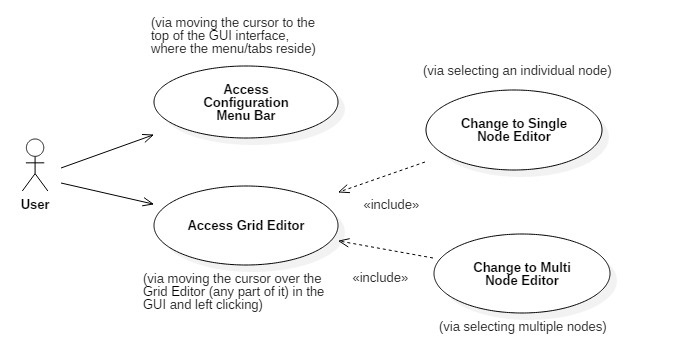
\includegraphics[width=170mm]{ComponetOverview.JPG}
		\caption{Use Case Diagram of "Basic" Component Overview \label{overflow}}
	\end{figure}
	
	% Subsubsections
	%----------------------------------------------------------------------------------------
	%	CONFIGURATION
	%----------------------------------------------------------------------------------------
	\subsubsection {Configuration Menu Bar}
	%\forceindent 
	The configuration menu bar will provide a simple interface via a horizontal menu bar at the top of the GUI that provides the user with various options on how they wish to configure the number of glasses, grid size, and checking/changing the pairing of the glasses. The number of glasses option will provide a simple diaglog box to enter the number of glasses/nodes the user wishes to use (and adjust the grid accordingly). The grid size option will also provide a diaglog box that allows the user to select a grid dimension (the grid dimensions will only be allowed if all the n nodes can fit within that space, otherwise a error will be thrown). There will able be a file option/tab that allows the user to open, create a new project, save, or save as for a project. %Finally, the checking/configuring glasses options will provide a simple display that shows how many glasses are connected, as well as having a drop down box option to pairing up glasses, which will then provide a dialog box to pair/edit glasses (via the receivers rotary switch on the glasses).
	The only inputs are from putting the cursor over the tabs and clicking on them to access their dialog boxes/displays as mentioned above. This component controls how the grid editor components dimensions are made up, and does have a component that it relies on to function properly. There should be some CPU-memory intensiveness for the tasks under this component, such as registering the number of Nodes/Glasses, changing the grid dimensions, and pairing glasses can all become intensive if the numbers are large enough, and general overhead due to GUI can occur. The general use-case of this component is shown in Figure 2.
	
	\begin{figure}[ht!]
		\centering
		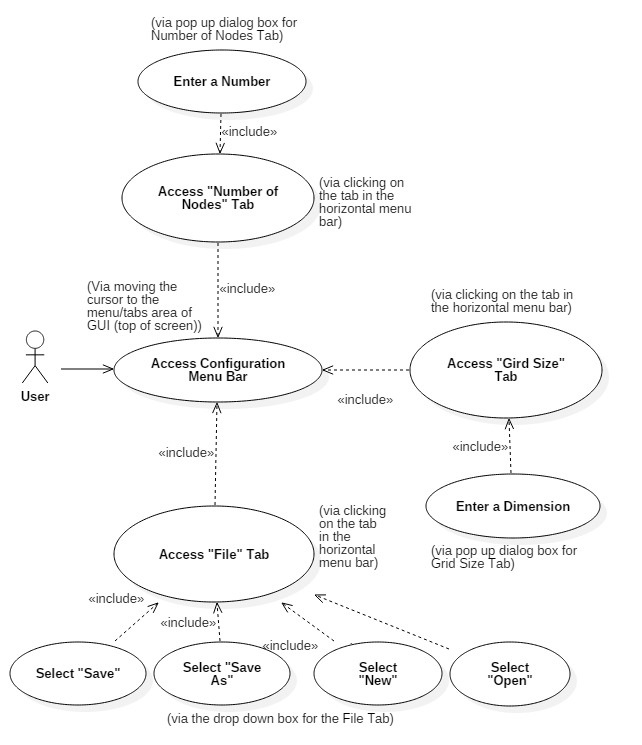
\includegraphics[width=170mm]{Configuration_Editor.JPG}
		\caption{Use Case Diagram of the Configuration Menu Bar \label{overflow}}
	\end{figure}
	
	%----------------------------------------------------------------------------------------
	%	SINGLE NODE EDITOR
	%----------------------------------------------------------------------------------------
	\subsubsection {Single Node Editor}
	%\forceindent 
	The Single Node Editor in the system software will allow the user to edit any individual node via a user interface. This means the user can hand pick various nodes and set specific colors to them. Thus the component allows the user to edit any individual node on the grid, choose a color via a color dialog box, and see the feedback via the grid Editor. The only inputs are from clicking on the individual node and then click on a color via the dialog box, and the output is displaying the color dialog box, and displaying the node with the chosen color. This component relies on the Grid Editor (who displays the nodes) for providing an interface. Constraints of this program are that it cannot be changed from this mode when editing a node is in process, and thus no other actions (in the system software) may be performed while editing a node (or the component will actually exit editing the node without applying any changes). There should not be any CPU-memory-intensiveness for task under this component, overhead may occur due to the GUI however. The general use-case of this component can be seen below in Figure 3.
	
	\begin{figure}[ht!]
		\centering
		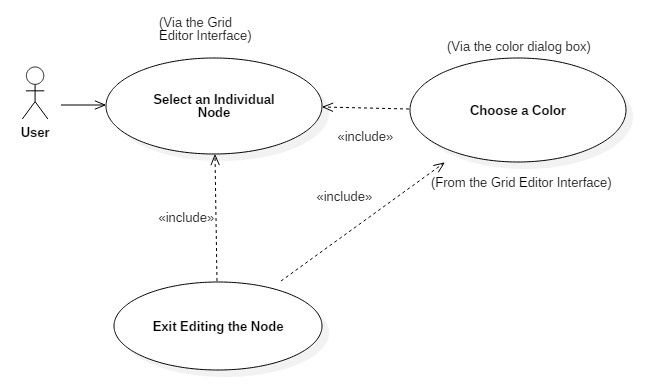
\includegraphics[width=150mm]{SingleNodeEditorDiagram.JPG}
		\caption{Use Case Diagram of Single Node Editor \label{overflow}}
	\end{figure}
	
	%----------------------------------------------------------------------------------------
	%	MULTI NODE EDITOR
	%----------------------------------------------------------------------------------------
	\subsubsection {Multi Node Editor}
	%\forceindent 
	The multi-node editor component is in charge of editing all the nodes within a grid. This component handles the selection of individual or multiple nodes. For example, the user may want to select a 20x20 sub-grid and change the color to green. The multi-node editor is responsible for allowing the user to select the 400 nodes. 
	
	This selection should be done in a way that is familiar to the user. One possible action-sequence starts with the user selecting a node in the corner of the sub-grid. Then, while holding down shift, the user would select the node in the corner of the sub-grid diagonal to the first node selected. The multi-node editor would be responsible to select all of the nodes in the sub-grid.
	
	After nodes are selected, the multi-node editor should give the user an opportunity to edit the properties (like color or on/off status) via the single-node editor. 
	
	The multi-node editor should also display a representation of the grid to the user via the GUI. See below for a mockup of the selection of a 2x2 sub-grid within an 8x8 grid.
	
	%----------------------------------------------------------------------------------------
	%	GRID EDITOR
	%----------------------------------------------------------------------------------------
	\subsubsection {Grid Editor}
	%\forceindent 
	The grid editor is responsible for the creation, selection, and manipulation of grids. Since the goal of this program is to create visualizations with the nodes, it is paramount to create the functionality to create and edit multiple grids. The grids work similar to a sprite animation; there is a collection of grids that will be cycled through in real-time with a slight delay. This can be used creatively to show animations.
	
	In regards to creation, the grid editor must take user input to create a new grid (perhaps a '+' button) and create corresponding data and GUI representations of the new grid. The user must also be able to delete grids. This component creates the ability to select single or multiple grids in a similar fashion to the multi-node editor.
	
	Additionally, the grid editor should allow the user to rearrange grids. This could take the form of dragging an individual grid to a different location within the array of grids. Navigation of the various grids is necessary. The grid editor will implement this functionality, perhaps with a scroll bar (see figure below).
	
	\begin{figure}[ht!]
		\centering
		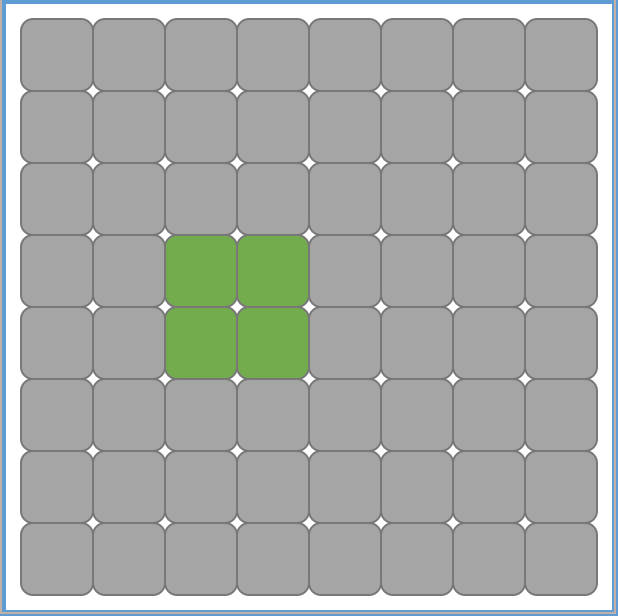
\includegraphics[width=80mm]{Grid.png}
		\caption{Grid Selection (green nodes are selected)}
	\end{figure}
	
	\begin{figure}[ht!]
		\centering
		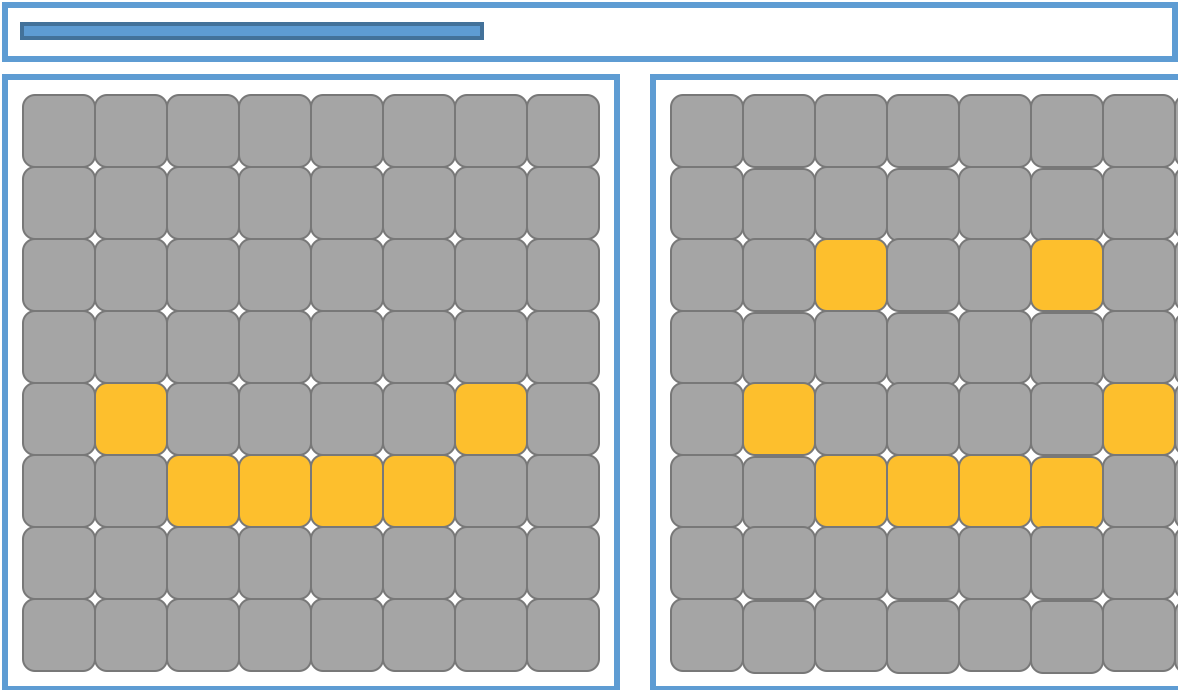
\includegraphics[width=100mm]{Multi-grid.png}
		\caption{Grid Editor w/ Scroll Bar}
	\end{figure}
	\clearpage
	
	
	%----------------------------------------------------------------------------------------
	%	COMPONENT RELATIONSHIP
	%----------------------------------------------------------------------------------------
	\subsection {Component Relationship}
	%\forceindent 	
	The character editor is responsible for the creation, editing, and saving of special grid formations, known as characters. By default, letters and numbers (and perhaps other standard keyboard characters) should exist in the character editor. Each character, like the letter 'A', has a corresponding grid that lights up the to represent the character.
	
	It is important to note that these default characters should be available regardless of the grid size. The character editor should allow the user to easily change the color of the character, regardless of whether it is a default character or not.
	
	Additionally, the character editor should allow for the creation of new characters. For example, ':)' might be saved as 'smiley face'. These user-created characters are intrinsically tied to their corresponding grid size. These new characters must also be saved for future use.
	

	
	\subsubsection{Animation Creator}
	The animation creator should implement the functionality to allow the user to create animations with characters. The animation creator should supply a text box for the user to input characters. The animation editor should then allow the user to pick an animation, like scrolling left to right, for the sequence of the characters.
	
	Based off of this, the animation creator should generate corresponding grids that simulates the animation of the characters. The user, if they so choose, should be able to edit the generated grids with the other components. 
	
	\subsubsection{File Generator}
	This component is responsible for outputting a text representation of the animations created in the program. The file must be in the "tan" format for use by the glasses and for future editing via this program.
	
	\subsubsection{Component Relationships}
	The first component that the user will interact with is the configuration component. Setup steps, like setting grid size, will be taken and will prepare the way for the other components to take over.
	
	After setup, a default grid of size n by m (as specified by the user to the configuration component) should be displayed. The grid editor is responsible for creating new grids and creating a multi-node editor instances to manage every new grid. When a node is deleted via the grid editor, the grid editor is responsible to destroy the multi-node editor for the deleted grid.
	
	When the user selects one or multiple nodes and chooses to edit their properties, the multi-node editor is responsible to call up the node editor. The node editor will then change the data representation of the edited node(s) which will then be reflected in the GUI as displayed by the multi-node editor.
	
	Alternatively, the user can use the animation creator to generate grids which can then be edited with the grid editor, multi-node editor, and node editor. The animation editor uses characters available through the character editor.
	
	See the use case diagram below.
	
	\begin{figure}[ht!]
		\centering
		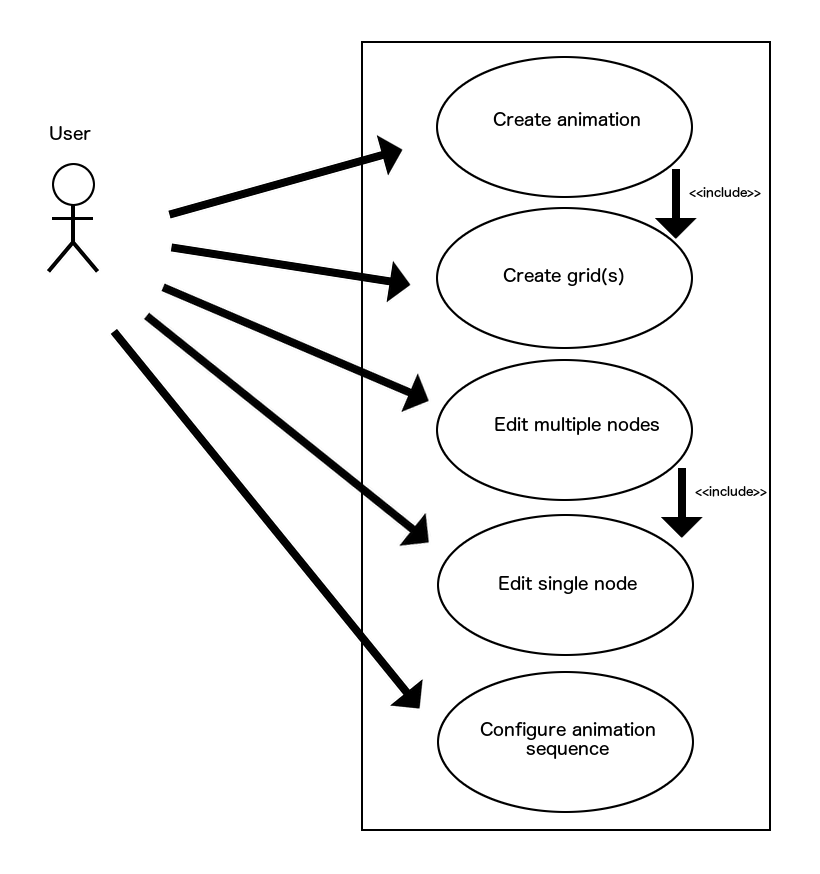
\includegraphics[width=100mm]{Relationship_Use.png}
		\caption{Use Cases}
	\end{figure}
	\clearpage
	
\newpage

	\section{Design Decisions}
	\subsection{Language Decisions}
	For our Goofy Lights Editor, we will be using Java. Java is convenient as it works easily across platforms, is very readable, and provides its own graphics package, the Swing package. Swing is designed to make APIs that work and look basically the same across all platforms that run Java. It's a package built into the language, no external libraries are needed. We considered using the Qt integration for Java, Qt Jambi, but we decided that this would add complexity without providing any real functionality. 
	
	\subsection{Complexity Decisions}
	When planning this project, several decisions were made to limit the scope and complexity of the final product. These decisions are detailed below. 
	\subsubsection{Constant Positions}
	We decided to support only constant positions of each node. If the nodes were free to move around during a performance, and the software needed to support such moving, the complexity would increase drastically. By limiting our editor to only allow a single configuration of nodes, per performance, we should be able to accomplish our goals. 
	\subsubsection{Grid Scalability}
	As stated previously, we will not allow changing of the grid during a performance. However, the grid should be configurable for the performance as a whole. The configuration component of our program will allow for this. The user will be able to set the dimensions of the grid to be used for the performance they are creating. This will mean that, in some cases, our editor will display a grid larger than the current number of nodes. In such a case the active nodes will be indicated. We decided that a solid rectangular grid will be the only supported configuration. The user will have to account for any unused nodes in the rectangle. Limiting the grid to be purely rectangular dramatically reduces the amount of options our editor would need to support, and we figure that a user will probably want a rectangular configuration in most if not all cases.
	%\pagebreak[4]
	\subsubsection{Letters and Default Animations}
	After viewing the current editor for the Tower of Lights, we decided that it would be convenient to add some default configurations for our editor. These would include static letters, as well as some built in animations such as the letters animating from one end of the grid to another. Adding this functionality should significantly improve ease of use, while not adding insurmountable complexity to our project. 
\newpage
	\section{Timeline}
	

	{ \setstretch{2.0}
		
	\scalebox{1}{
		
		\begin{tabular}{r |@{\tline} l}
			
			March 6 & Design Specifications v1\\
			
			March 21 & Begin Version 1 of GoofyLights\\
			March 23 & Unit Testing of Version 1\\
			March 28 & Develop Single Node Editor\\
			March 30 & Unit Testing Single Node Editor\\
			April 4 & Develop Multiple Node Editor\\
			April 6 & Unit Testing Multiple Node Editor\\
			April 11 & Develop Grid Editor\\
			April 13 & Unit Testing Grid Editor\\
			April 18 & Extra time to catch up or add additional features\\
			April 20 & Goal Specifications for System Testing\\
			April 25 & System Testing\\
			May 1 & Preparation for Final Presentation\\
			May 4 & GoofyLights Final Presentation\\
			
		\end{tabular}
		
		}
	
	}

\end{document}
